% Graphic for TeX using PGF
% Title: C:\Users\CAMUGLIAL_INFO\Desktop\Diplome\Diplome\_Documentation\Diagrammes\Gpx2Sql
% Creator: Dia v0.97.2
% CreationDate: Mon Jun 12 07:58:56 2017
% For: CAMUGLIAL_INFO
% \usepackage{tikz}
% The following commands are not supported in PSTricks at present
% We define them conditionally, so when they are implemented,
% this pgf file will use them.
\ifx\du\undefined
  \newlength{\du}
\fi
\setlength{\du}{15\unitlength}
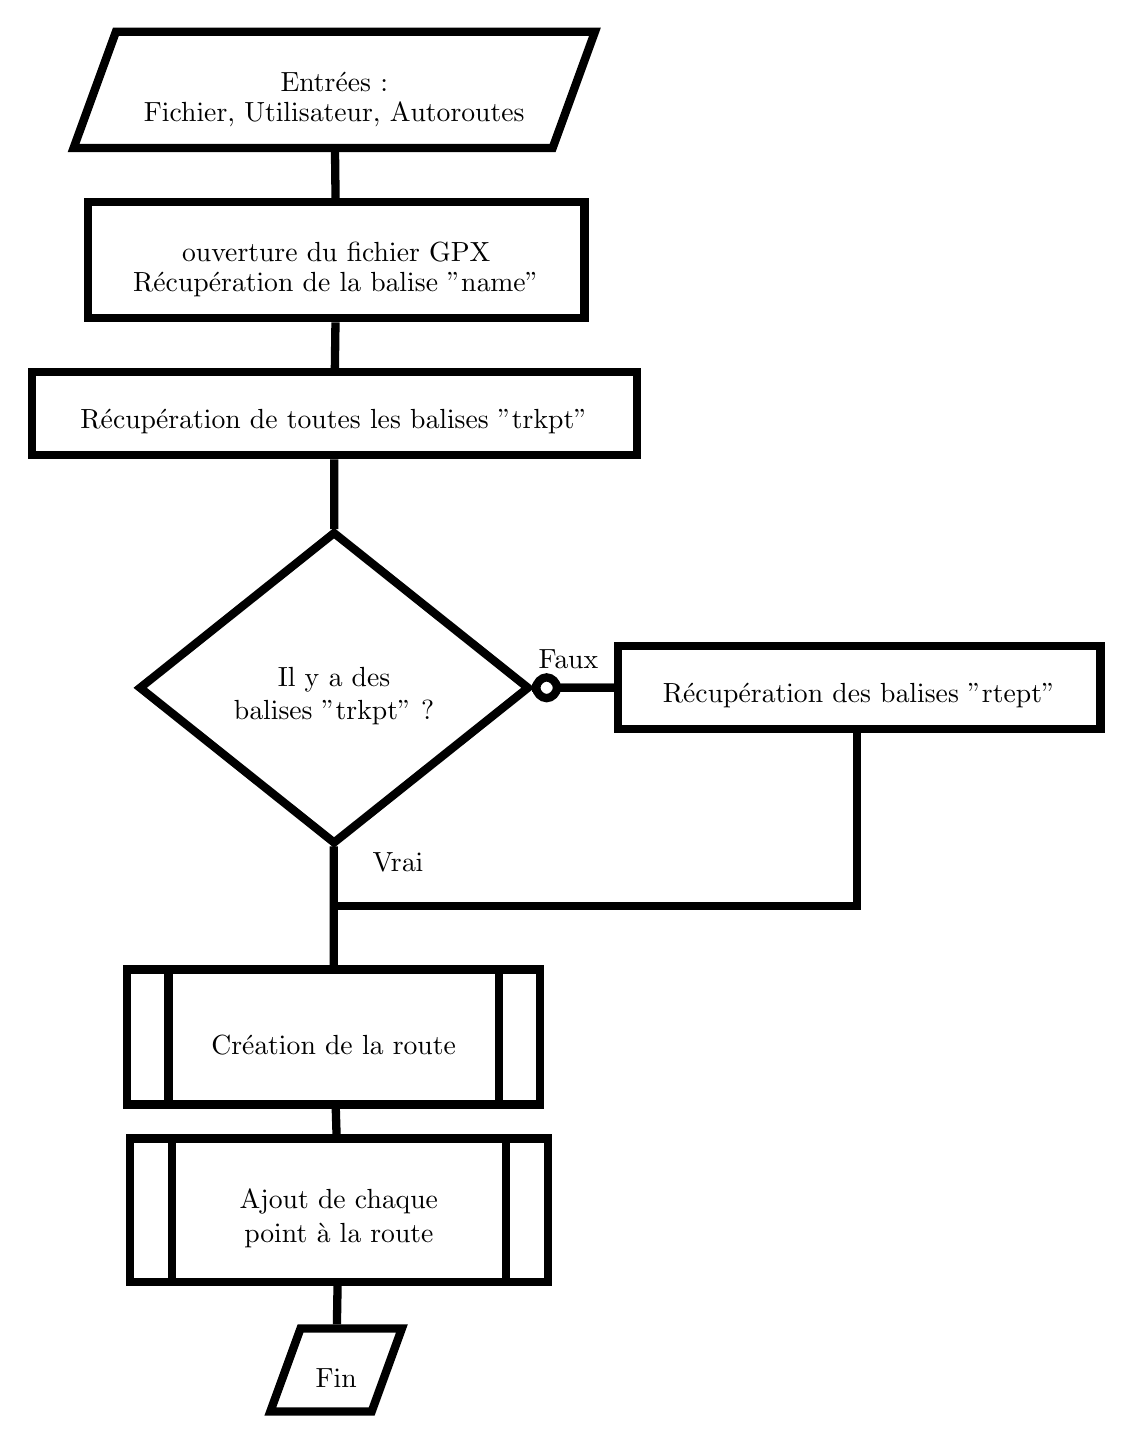
\begin{tikzpicture}
\pgftransformxscale{1.000000}
\pgftransformyscale{-1.000000}
\definecolor{dialinecolor}{rgb}{0.000000, 0.000000, 0.000000}
\pgfsetstrokecolor{dialinecolor}
\definecolor{dialinecolor}{rgb}{1.000000, 1.000000, 1.000000}
\pgfsetfillcolor{dialinecolor}
\definecolor{dialinecolor}{rgb}{1.000000, 1.000000, 1.000000}
\pgfsetfillcolor{dialinecolor}
\fill (17.739817\du,-14.850000\du)--(29.279669\du,-14.850000\du)--(28.260552\du,-12.050000\du)--(16.720700\du,-12.050000\du)--cycle;
\pgfsetlinewidth{0.200000\du}
\pgfsetdash{}{0pt}
\pgfsetdash{}{0pt}
\pgfsetmiterjoin
\definecolor{dialinecolor}{rgb}{0.000000, 0.000000, 0.000000}
\pgfsetstrokecolor{dialinecolor}
\draw (17.739817\du,-14.850000\du)--(29.279669\du,-14.850000\du)--(28.260552\du,-12.050000\du)--(16.720700\du,-12.050000\du)--cycle;
% setfont left to latex
\definecolor{dialinecolor}{rgb}{0.000000, 0.000000, 0.000000}
\pgfsetstrokecolor{dialinecolor}
\node at (23.000185\du,-13.655000\du){Entrées : };
% setfont left to latex
\definecolor{dialinecolor}{rgb}{0.000000, 0.000000, 0.000000}
\pgfsetstrokecolor{dialinecolor}
\node at (23.000185\du,-12.855000\du){Fichier, Utilisateur, Autoroutes};
\definecolor{dialinecolor}{rgb}{1.000000, 1.000000, 1.000000}
\pgfsetfillcolor{dialinecolor}
\fill (17.075000\du,-10.750000\du)--(17.075000\du,-7.950000\du)--(29.025000\du,-7.950000\du)--(29.025000\du,-10.750000\du)--cycle;
\pgfsetlinewidth{0.200000\du}
\pgfsetdash{}{0pt}
\pgfsetdash{}{0pt}
\pgfsetmiterjoin
\definecolor{dialinecolor}{rgb}{0.000000, 0.000000, 0.000000}
\pgfsetstrokecolor{dialinecolor}
\draw (17.075000\du,-10.750000\du)--(17.075000\du,-7.950000\du)--(29.025000\du,-7.950000\du)--(29.025000\du,-10.750000\du)--cycle;
% setfont left to latex
\definecolor{dialinecolor}{rgb}{0.000000, 0.000000, 0.000000}
\pgfsetstrokecolor{dialinecolor}
\node at (23.050000\du,-9.555000\du){ouverture du fichier GPX};
% setfont left to latex
\definecolor{dialinecolor}{rgb}{0.000000, 0.000000, 0.000000}
\pgfsetstrokecolor{dialinecolor}
\node at (23.050000\du,-8.755000\du){Récupération de la balise "name"};
\definecolor{dialinecolor}{rgb}{1.000000, 1.000000, 1.000000}
\pgfsetfillcolor{dialinecolor}
\fill (15.715000\du,-6.650000\du)--(15.715000\du,-4.650000\du)--(30.285000\du,-4.650000\du)--(30.285000\du,-6.650000\du)--cycle;
\pgfsetlinewidth{0.200000\du}
\pgfsetdash{}{0pt}
\pgfsetdash{}{0pt}
\pgfsetmiterjoin
\definecolor{dialinecolor}{rgb}{0.000000, 0.000000, 0.000000}
\pgfsetstrokecolor{dialinecolor}
\draw (15.715000\du,-6.650000\du)--(15.715000\du,-4.650000\du)--(30.285000\du,-4.650000\du)--(30.285000\du,-6.650000\du)--cycle;
% setfont left to latex
\definecolor{dialinecolor}{rgb}{0.000000, 0.000000, 0.000000}
\pgfsetstrokecolor{dialinecolor}
\node at (23.000000\du,-5.455000\du){Récupération de toutes les balises "trkpt"};
\definecolor{dialinecolor}{rgb}{1.000000, 1.000000, 1.000000}
\pgfsetfillcolor{dialinecolor}
\fill (22.995519\du,-2.774080\du)--(27.666438\du,0.952728\du)--(22.995519\du,4.679536\du)--(18.324600\du,0.952728\du)--cycle;
\pgfsetlinewidth{0.200000\du}
\pgfsetdash{}{0pt}
\pgfsetdash{}{0pt}
\pgfsetmiterjoin
\definecolor{dialinecolor}{rgb}{0.000000, 0.000000, 0.000000}
\pgfsetstrokecolor{dialinecolor}
\draw (22.995519\du,-2.774080\du)--(27.666438\du,0.952728\du)--(22.995519\du,4.679536\du)--(18.324600\du,0.952728\du)--cycle;
% setfont left to latex
\definecolor{dialinecolor}{rgb}{0.000000, 0.000000, 0.000000}
\pgfsetstrokecolor{dialinecolor}
\node at (22.995519\du,0.747728\du){Il y a des};
% setfont left to latex
\definecolor{dialinecolor}{rgb}{0.000000, 0.000000, 0.000000}
\pgfsetstrokecolor{dialinecolor}
\node at (22.995519\du,1.547728\du){ balises "trkpt" ?};
\definecolor{dialinecolor}{rgb}{1.000000, 1.000000, 1.000000}
\pgfsetfillcolor{dialinecolor}
\fill (29.841200\du,-0.050000\du)--(29.841200\du,1.950000\du)--(41.458700\du,1.950000\du)--(41.458700\du,-0.050000\du)--cycle;
\pgfsetlinewidth{0.200000\du}
\pgfsetdash{}{0pt}
\pgfsetdash{}{0pt}
\pgfsetmiterjoin
\definecolor{dialinecolor}{rgb}{0.000000, 0.000000, 0.000000}
\pgfsetstrokecolor{dialinecolor}
\draw (29.841200\du,-0.050000\du)--(29.841200\du,1.950000\du)--(41.458700\du,1.950000\du)--(41.458700\du,-0.050000\du)--cycle;
% setfont left to latex
\definecolor{dialinecolor}{rgb}{0.000000, 0.000000, 0.000000}
\pgfsetstrokecolor{dialinecolor}
\node at (35.649950\du,1.145000\du){Récupération des balises "rtept"};
\pgfsetlinewidth{0.200000\du}
\pgfsetdash{}{0pt}
\pgfsetdash{}{0pt}
\pgfsetbuttcap
\pgfsetmiterjoin
\pgfsetlinewidth{0.200000\du}
\pgfsetbuttcap
\pgfsetmiterjoin
\pgfsetdash{}{0pt}
\definecolor{dialinecolor}{rgb}{1.000000, 1.000000, 1.000000}
\pgfsetfillcolor{dialinecolor}
\fill (18.009200\du,7.739760\du)--(18.009200\du,10.989760\du)--(27.959200\du,10.989760\du)--(27.959200\du,7.739760\du)--cycle;
\definecolor{dialinecolor}{rgb}{0.000000, 0.000000, 0.000000}
\pgfsetstrokecolor{dialinecolor}
\draw (18.009200\du,7.739760\du)--(18.009200\du,10.989760\du)--(27.959200\du,10.989760\du)--(27.959200\du,7.739760\du)--cycle;
\pgfsetbuttcap
\pgfsetmiterjoin
\pgfsetdash{}{0pt}
\definecolor{dialinecolor}{rgb}{0.000000, 0.000000, 0.000000}
\pgfsetstrokecolor{dialinecolor}
\draw (19.004200\du,7.739760\du)--(19.004200\du,10.989760\du);
\pgfsetbuttcap
\pgfsetmiterjoin
\pgfsetdash{}{0pt}
\definecolor{dialinecolor}{rgb}{0.000000, 0.000000, 0.000000}
\pgfsetstrokecolor{dialinecolor}
\draw (26.964200\du,7.739760\du)--(26.964200\du,10.989760\du);
% setfont left to latex
\definecolor{dialinecolor}{rgb}{0.000000, 0.000000, 0.000000}
\pgfsetstrokecolor{dialinecolor}
\node at (22.984200\du,9.564760\du){Création de la route};
\pgfsetlinewidth{0.200000\du}
\pgfsetdash{}{0pt}
\pgfsetdash{}{0pt}
\pgfsetbuttcap
\pgfsetmiterjoin
\pgfsetlinewidth{0.200000\du}
\pgfsetbuttcap
\pgfsetmiterjoin
\pgfsetdash{}{0pt}
\definecolor{dialinecolor}{rgb}{1.000000, 1.000000, 1.000000}
\pgfsetfillcolor{dialinecolor}
\fill (18.076700\du,11.812500\du)--(18.076700\du,15.262500\du)--(28.145450\du,15.262500\du)--(28.145450\du,11.812500\du)--cycle;
\definecolor{dialinecolor}{rgb}{0.000000, 0.000000, 0.000000}
\pgfsetstrokecolor{dialinecolor}
\draw (18.076700\du,11.812500\du)--(18.076700\du,15.262500\du)--(28.145450\du,15.262500\du)--(28.145450\du,11.812500\du)--cycle;
\pgfsetbuttcap
\pgfsetmiterjoin
\pgfsetdash{}{0pt}
\definecolor{dialinecolor}{rgb}{0.000000, 0.000000, 0.000000}
\pgfsetstrokecolor{dialinecolor}
\draw (19.083575\du,11.812500\du)--(19.083575\du,15.262500\du);
\pgfsetbuttcap
\pgfsetmiterjoin
\pgfsetdash{}{0pt}
\definecolor{dialinecolor}{rgb}{0.000000, 0.000000, 0.000000}
\pgfsetstrokecolor{dialinecolor}
\draw (27.138575\du,11.812500\du)--(27.138575\du,15.262500\du);
% setfont left to latex
\definecolor{dialinecolor}{rgb}{0.000000, 0.000000, 0.000000}
\pgfsetstrokecolor{dialinecolor}
\node at (23.111075\du,13.337500\du){Ajout de chaque };
% setfont left to latex
\definecolor{dialinecolor}{rgb}{0.000000, 0.000000, 0.000000}
\pgfsetstrokecolor{dialinecolor}
\node at (23.111075\du,14.137500\du){point à la route};
\definecolor{dialinecolor}{rgb}{1.000000, 1.000000, 1.000000}
\pgfsetfillcolor{dialinecolor}
\fill (22.188740\du,16.385700\du)--(24.629917\du,16.385700\du)--(23.901976\du,18.385700\du)--(21.460800\du,18.385700\du)--cycle;
\pgfsetlinewidth{0.200000\du}
\pgfsetdash{}{0pt}
\pgfsetdash{}{0pt}
\pgfsetmiterjoin
\definecolor{dialinecolor}{rgb}{0.000000, 0.000000, 0.000000}
\pgfsetstrokecolor{dialinecolor}
\draw (22.188740\du,16.385700\du)--(24.629917\du,16.385700\du)--(23.901976\du,18.385700\du)--(21.460800\du,18.385700\du)--cycle;
% setfont left to latex
\definecolor{dialinecolor}{rgb}{0.000000, 0.000000, 0.000000}
\pgfsetstrokecolor{dialinecolor}
\node at (23.045358\du,17.580700\du){Fin};
\pgfsetlinewidth{0.200000\du}
\pgfsetdash{}{0pt}
\pgfsetdash{}{0pt}
\pgfsetbuttcap
{
\definecolor{dialinecolor}{rgb}{0.000000, 0.000000, 0.000000}
\pgfsetfillcolor{dialinecolor}
% was here!!!
\definecolor{dialinecolor}{rgb}{0.000000, 0.000000, 0.000000}
\pgfsetstrokecolor{dialinecolor}
\draw (27.766438\du,0.951700\du)--(29.740970\du,0.951274\du);
}
\definecolor{dialinecolor}{rgb}{0.000000, 0.000000, 0.000000}
\pgfsetstrokecolor{dialinecolor}
\draw (28.366438\du,0.951570\du)--(29.740970\du,0.951274\du);
\pgfsetlinewidth{0.200000\du}
\pgfsetdash{}{0pt}
\pgfsetmiterjoin
\pgfsetbuttcap
\definecolor{dialinecolor}{rgb}{1.000000, 1.000000, 1.000000}
\pgfsetfillcolor{dialinecolor}
\pgfpathmoveto{\pgfpoint{27.866438\du}{0.951678\du}}
\pgfpathcurveto{\pgfpoint{27.866411\du}{0.826678\du}}{\pgfpoint{27.991384\du}{0.701651\du}}{\pgfpoint{28.116384\du}{0.701624\du}}
\pgfpathcurveto{\pgfpoint{28.241384\du}{0.701597\du}}{\pgfpoint{28.366411\du}{0.826570\du}}{\pgfpoint{28.366438\du}{0.951570\du}}
\pgfpathcurveto{\pgfpoint{28.366465\du}{1.076570\du}}{\pgfpoint{28.241492\du}{1.201597\du}}{\pgfpoint{28.116492\du}{1.201624\du}}
\pgfpathcurveto{\pgfpoint{27.991492\du}{1.201651\du}}{\pgfpoint{27.866465\du}{1.076678\du}}{\pgfpoint{27.866438\du}{0.951678\du}}
\pgfusepath{fill}
\definecolor{dialinecolor}{rgb}{0.000000, 0.000000, 0.000000}
\pgfsetstrokecolor{dialinecolor}
\pgfpathmoveto{\pgfpoint{27.866438\du}{0.951678\du}}
\pgfpathcurveto{\pgfpoint{27.866411\du}{0.826678\du}}{\pgfpoint{27.991384\du}{0.701651\du}}{\pgfpoint{28.116384\du}{0.701624\du}}
\pgfpathcurveto{\pgfpoint{28.241384\du}{0.701597\du}}{\pgfpoint{28.366411\du}{0.826570\du}}{\pgfpoint{28.366438\du}{0.951570\du}}
\pgfpathcurveto{\pgfpoint{28.366465\du}{1.076570\du}}{\pgfpoint{28.241492\du}{1.201597\du}}{\pgfpoint{28.116492\du}{1.201624\du}}
\pgfpathcurveto{\pgfpoint{27.991492\du}{1.201651\du}}{\pgfpoint{27.866465\du}{1.076678\du}}{\pgfpoint{27.866438\du}{0.951678\du}}
\pgfusepath{stroke}
\pgfsetlinewidth{0.200000\du}
\pgfsetdash{}{0pt}
\pgfsetdash{}{0pt}
\pgfsetbuttcap
{
\definecolor{dialinecolor}{rgb}{0.000000, 0.000000, 0.000000}
\pgfsetfillcolor{dialinecolor}
% was here!!!
\definecolor{dialinecolor}{rgb}{0.000000, 0.000000, 0.000000}
\pgfsetstrokecolor{dialinecolor}
\draw (23.018409\du,-11.950037\du)--(23.031775\du,-10.849963\du);
}
\pgfsetlinewidth{0.200000\du}
\pgfsetdash{}{0pt}
\pgfsetdash{}{0pt}
\pgfsetbuttcap
{
\definecolor{dialinecolor}{rgb}{0.000000, 0.000000, 0.000000}
\pgfsetfillcolor{dialinecolor}
% was here!!!
\definecolor{dialinecolor}{rgb}{0.000000, 0.000000, 0.000000}
\pgfsetstrokecolor{dialinecolor}
\draw (23.029730\du,-7.850037\du)--(23.014856\du,-6.749341\du);
}
\pgfsetlinewidth{0.200000\du}
\pgfsetdash{}{0pt}
\pgfsetdash{}{0pt}
\pgfsetbuttcap
{
\definecolor{dialinecolor}{rgb}{0.000000, 0.000000, 0.000000}
\pgfsetfillcolor{dialinecolor}
% was here!!!
\definecolor{dialinecolor}{rgb}{0.000000, 0.000000, 0.000000}
\pgfsetstrokecolor{dialinecolor}
\draw (22.999253\du,-4.549814\du)--(22.998114\du,-2.871728\du);
}
\pgfsetlinewidth{0.200000\du}
\pgfsetdash{}{0pt}
\pgfsetdash{}{0pt}
\pgfsetbuttcap
{
\definecolor{dialinecolor}{rgb}{0.000000, 0.000000, 0.000000}
\pgfsetfillcolor{dialinecolor}
% was here!!!
\definecolor{dialinecolor}{rgb}{0.000000, 0.000000, 0.000000}
\pgfsetstrokecolor{dialinecolor}
\draw (22.990376\du,4.775212\du)--(22.986510\du,7.647851\du);
}
\pgfsetlinewidth{0.200000\du}
\pgfsetdash{}{0pt}
\pgfsetdash{}{0pt}
\pgfsetbuttcap
{
\definecolor{dialinecolor}{rgb}{0.000000, 0.000000, 0.000000}
\pgfsetfillcolor{dialinecolor}
% was here!!!
\definecolor{dialinecolor}{rgb}{0.000000, 0.000000, 0.000000}
\pgfsetstrokecolor{dialinecolor}
\draw (23.036641\du,11.089479\du)--(23.059532\du,11.842324\du);
}
\pgfsetlinewidth{0.200000\du}
\pgfsetdash{}{0pt}
\pgfsetdash{}{0pt}
\pgfsetbuttcap
{
\definecolor{dialinecolor}{rgb}{0.000000, 0.000000, 0.000000}
\pgfsetfillcolor{dialinecolor}
% was here!!!
\definecolor{dialinecolor}{rgb}{0.000000, 0.000000, 0.000000}
\pgfsetstrokecolor{dialinecolor}
\draw (23.079909\du,15.362483\du)--(23.064138\du,16.286013\du);
}
\pgfsetlinewidth{0.200000\du}
\pgfsetdash{}{0pt}
\pgfsetdash{}{0pt}
\pgfsetmiterjoin
\pgfsetbuttcap
{
\definecolor{dialinecolor}{rgb}{0.000000, 0.000000, 0.000000}
\pgfsetfillcolor{dialinecolor}
% was here!!!
{\pgfsetcornersarced{\pgfpoint{0.000000\du}{0.000000\du}}\definecolor{dialinecolor}{rgb}{0.000000, 0.000000, 0.000000}
\pgfsetstrokecolor{dialinecolor}
\draw (35.650000\du,1.950000\du)--(35.600000\du,1.950000\du)--(35.600000\du,6.211530\du)--(22.988400\du,6.211530\du);
}}
% setfont left to latex
\definecolor{dialinecolor}{rgb}{0.000000, 0.000000, 0.000000}
\pgfsetstrokecolor{dialinecolor}
\node[anchor=west] at (23.600000\du,5.150000\du){Vrai};
% setfont left to latex
\definecolor{dialinecolor}{rgb}{0.000000, 0.000000, 0.000000}
\pgfsetstrokecolor{dialinecolor}
\node[anchor=west] at (27.600000\du,0.250000\du){Faux};
\end{tikzpicture}
